\section{Algoritmi risolutivi}
In questa sezione esamineremo alcuni algoritmi risolutivi proposti per la risoluzione del problema della determinazione della massima bisimulazione su un grafo. Come risulterà evidente nel seguito viene sfruttata ampiamente l'equivalenza tra bisimulazione massima e RCSP dimostrata nella sezione precedente.

\subsection{Minimizzazione di automi a stati finiti}
Esaminiamo innanzitutto l'algoritmo risolutivo per una versione semplificata del problema della determinazione della bisimulazione massima, ovvero la minimizzazione di un'automa a stati finiti, presentato in \cite{hopcroft} nel 1971. Sebbene questa soluzione non sia generale, ha fornito alcuni spunti fondamentali per l'ideazione di algoritmi risolutivi più completi, che verranno presentati nel seguito del lavoro.

\subsubsection{Alcune nozioni fondamentali}
Innanzitutto definiamo il concetto di \emph{automa}, chiaramente centrale nella descrizione del problema:
\begin{definition}
    Consideriamo i seguenti oggetti:
    \begin{itemize}
        \item Un insieme finito $I$ detto \emph{insieme degli ingressi};
        \item Un insieme finito $S$ detto \emph{insieme degli stati}, ad ogni stato è associata un'unica uscita;
        \item Un insieme finito $F \subseteq S$ detto \emph{insieme degli stati finali};
        \item Una funzione $\delta: S \times I E S$ detta \emph{funzione di trasferimento}.
    \end{itemize}
    Chiameremo $A = (S,I,\delta,F)$ \emph{automa}. Useremo la notazione $Out(x)$ per indicare l'output corrispondente allo stato $x$.
\end{definition}
Possiamo rappresentare un'automa con una tabella degli stati, in cui ogni riga rappresenta uno stato, ogni colonna un ingresso, ed ogni cella contiene il nuovo stato del sistema quando, nel momento in cui il sistema si trova nello stato corrispondente alla riga, si inserisce l'ingresso corrispondente alla colonna.In alternativa possiamo utilizzare una rappresentazione grafica, in cui ogni stato è descritto da un cerchio contenente il nome dello stato, e le transizioni tra stati sono descritte da frecce, sulle quali viene specificato l'ingresso che ha innescato la transizione.\\
\begin{example}
    Nella Tabella \ref{fig:tab_automata} è rappresentato un'automa che cambia stato ($A E B$, $B E C$) solamente se l'ingresso è ``1'', e lo stato non è ``$C$''. In qualsiasi altro caso lo stato non cambia.
    \begin{table}[ht]
        \centering
        \begin{tabular}{ c | c c }
            \hline
            & 0 & 1\\
            \hline
            a[0] & a & b \\
            b[0] & b & c \\
            c[1] & c & c \\
            \hline
          \end{tabular}
        \caption{Rappresentazione tabellare di un'automa}
        \label{fig:tab_automata}
    \end{table}
    \label{exa:automata_tab}
\end{example}
\begin{example}
    Nella Figura \ref{fig:automata} è rappresentato lo stesso automa dell'Esempio \ref{exa:automata_tab}.
    \begin{figure}[hb]
        \centering
        \begin{tikzpicture}[->,>=stealth',shorten >=1pt,auto,node distance=3.5cm,
            scale = 1,transform shape]
            \node[state] (a) {$a[0]$};
            \node[state] (b) [right of=a] {$b[0]$};
            \node[state] (c) [right of=b] {$c[1]$};

            \path (a) edge              node {$1$} (b)
                  (b) edge              node {$1$} (c)
                  (a) edge [loop above]             node {$0$} (a)
                  (b) edge [loop above]             node {$0$} (b)
                  (c) edge [loop above]              node {$0/1$} (c);
        \end{tikzpicture}
        \caption{Rappresentazione grafica di un'automa}
        \label{fig:automata}
    \end{figure}
\end{example}
In alcuni automi è possibile individuare stati che ``si comportano in modo simile''. Informalmente, il sistema si comporta in modo simile quando riceve in input un ingresso qualsiasi, e si trova in uno degli stati presi in esame. Diamo un esempio di questa situazione:
\begin{example}
    \begin{figure}[b]
        \centering
        \begin{tikzpicture}[->,>=stealth',shorten >=1pt,auto,node distance=3.5cm,
            scale = 1,transform shape]
            \node[state] (a) {$a[0]$};
            \node[state] (b) [right of=a] {$b[1]$};
            \node[state] (c) [right of=b] {$c[1]$};

            \path (a) edge              node {$1$} (b)
                  (b) edge [bend right]             node {$1$} (c)
                  (c) edge [bend right]             node {$1$} (b)
                  (a) edge [loop above]             node {$0$} (a)
                  (b) edge [loop above]             node {$0$} (b)
                  (c) edge [loop above]             node {$0$} (c);
        \end{tikzpicture}
        \caption{Automa contenente stati equivalenti}
        \label{fig:automata_eq}
    \end{figure}
    Consideriamo gli stati dell'automa rappresentato graficamente nella Figura \ref{fig:automata_eq}. Supponiamo di accorpare gli stati $B,C$ in un unico stato, che chiamiamo $B'$. Se ci interessiamo solamente alla sequenza di output ed all'eventuale raggiungimento di uno stato finale, il nuovo automa risulta indistinguibile dal primo.
\end{example}
Proponiamo la definizione formale di equivalenza tra stati che viene utilizzata in \cite{hopcroft}. Nel seguito ne dedurremo un'altra, che consente di stabilire un parallelo con gli argomenti trattati nella Sezione \ref{sec:base}.
\begin{definition}
    \label{def:equivalent_states}
    Sia $I^*$ l'insieme di tutte le sequenze di input di lunghezza finita. Sia $\delta^* : S \times I^*$ la funzione di transizione ``iterata''. Diremo che due stati $x,y$ sono equivalenti (con la notazione ``$x \sim y$'') se e soltanto se valgono congiuntamente le seguenti condizioni:
    \begin{enumerate}
        \item $Out(x) = Out(y)$;
        \item $\forall i^* \in I^*,\,\, \delta^*(x,i^*) \in F \iff \delta^*(y,i^*) \in F$.
    \end{enumerate}
\end{definition}
\accente evidente che individuare g
li stati equivalenti consente di minimizzare il sistema, preservando al tempo stesso i risultati ottenuti. In questo lavoro non illustreremo cosa comporta questa definizione, e perchè è importante che per qualsiasi stringa di lunghezza finita si giunga ad uno stato finale partendo da due stati supposti equivalenti.
\begin{observation}
    La relazione ``$\sim$'' così definita è una relazione di equivalenza sull'insieme degli stati di un'automa.
\end{observation}
La seguente proposizione sarà utile per formulare il problema con la terminologia esposta nella Sezione \ref{sec:rscp}:
\begin{proposition}
    \label{prop:equivalent_states}
    Due stati $x,y$ sono equivalenti nel senso della definizione \ref{def:equivalent_states} se e solo se
    \begin{gather}
        \forall i \in I, \quad \delta(x,i) \sim \delta(y,i)
    \end{gather}
    e $Out(x) = Out(y)$.
\end{proposition}
\begin{proof2}
    Supponiamo che $\exists i \in I : \delta(x,i) \not\sim \delta(y,i)$. Allora, ad esempio:
    \begin{gather*}
        \exists i^* \in I^* : \delta^*(\delta(x,i),i^*) = \delta^*(x,ii^*) \in F, \,\, \delta^*(\delta(y,i),i^*) = \delta^*(y,ii^*) \notin F
    \end{gather*}
    Quindi, per l'esistenza della stringa $ii^*$ si ha $x \not\sim y$. La dimostrazione è speculare se $\exists i^* \in I^* : \delta^*(x,ii^*) \notin F, \delta^*(y,ii^*) \in F$.\\
    Ora supponiamo che valga la (1). E' chiaro che $\forall i^* \in I^*, \forall i \in I$ si ha che
    \begin{gather*}
        \delta^*(x,ii^*) \sim \delta^*(y,ii^*)
    \end{gather*}
    e quindi $x \sim y$.
\end{proof2}
\begin{proposition}
    La relazione ``$\sim$'' con la formulazione dell'Osservazione \ref{prop:equivalent_states} è una bisimulazione sull'insieme degli stati di un'automa, se si considera la relazione binaria $\displaystyle E \,\,\coloneqq \bigcup_{i \in I, x \in S} \{(x,\delta(x,i))\}$.
\end{proposition}
\begin{proof2}
    Supponiamo che $x \sim y$. Sia $x E x'$, cioè $\exists i \in I : x' = \delta(x,i)$. Sia $y' = \delta(y,i) \implies y E y'$. Allora, per l'Osservazione \ref{prop:equivalent_states}, $x' \sim y'$.\\
    Chiaramente lo stesso argomento vale in modo speculare.
\end{proof2}
Osserviamo che nella definizione di ``$E$'' si perde un'informazione importante, cioè il fatto che per $i \in I$ fissato $\delta_i(x) \coloneqq \delta(x,i)$ è una funzione, ovvero l'insieme immagine di ogni $x \in S$ ha cardinalità 1. L'algoritmo di Hopcroft sfrutta questa proprietà nel procedimento che consente di migliorare l'algoritmo banale che verrà discusso nel seguito del lavoro.\\
Possiamo definire la \emph{minimizzazione per stati equivalenti} di un'automa a stati finiti:
\begin{definition}\label{def:minim_eq_states}
    Sia $A = (S,I,\delta,F)$ un'automa. Chiameremo \emph{minimizzazione per stati equivalenti} l'automa $A = (\widetilde{S}, I, \widetilde{\delta}, \widetilde{F})$ dove
    \begin{itemize}
        \item $\widetilde{S} =$ ``l'insieme delle classi di equivalenza di $\sim$ su $S$'';
        \item $\widetilde{\delta} : (\widetilde{S} \times I) E \widetilde{S}, \quad \delta(i, x) = y \implies \widetilde{\delta}(i,\widetilde{x}) = \widetilde{y}$, dove $x,y \in S, i \in I$, e $\widetilde{x}, \widetilde{y} \in \widetilde{S}$ sono rispettivamente le classi di equivalenza di ``$\sim$'' a cui appartengono $x,y$;
        \item $\widetilde{F} =$ ``l'insieme delle classi di equivalenza di $\sim$ su $F$'';
    \end{itemize}
\end{definition}
Prima di concludere l'esposizione delle nozioni preliminari è necessario dimostrare un risultato interessante che lega il problema della minimizzazzione di un'automa a stati finiti con quanto è stato presentato nella sezione \ref{sec:rscp}. A questo scopo dimostriamo i seguenti lemmi, che consentono di dimostrare tale legame in modo agevole:
\begin{lemma}
    \label{lem:part_stab_stesso_blocco}
    Sia $A = (S,I,F,\delta)$ un'automa. Sia $\widehat{S}$ una partizione di $S$ stabile rispetto alle funzioni $\delta_i, \forall i \in I$. Allora $\forall (x,y) \in S \times S$ tali che $[x]_{\widehat{S}} = [y]_{\widehat{S}}$ si ha che $\forall i^* \in I^*$
    \begin{gather*}
        [\delta^*(x,i^*)]_{\widehat{S}} = [\delta^*(y,i^*)]_{\widehat{S}}
    \end{gather*}
\end{lemma}
\begin{proof2}
    Procediamo per induzione su $i^*$. Inizialmente i due stati si trovano nello stesso blocco. Ora supponiamo che dopo l'inserimento dell' $(n-1)$-esimo simbolo di $i^*$ i due stati $x_{n-1}, y_{n-1}$ in cui si trova l'automa appartengano ancora allo stesso blocco. La partizione è stabile rispetto alla funzione $\delta_i$, dove $i$ è l' $n$-esimo simbolo di $i^*$, quindi tutto il blocco $[x_{n-1}]_{\widehat{S}} = [y_{n-1}]_{\widehat{S}}\,\,$ è contenuto all'interno dell'insieme $\delta_i^{-1}([\delta_i(x_{n-1})]_{\widehat{S}}) = \delta_i^{-1}([x_n]_{\widehat{S}})$. Quindi $\delta_i(y_{n-1}) \in \delta_i^{-1}([x_n]_{\widehat{S}})$, e dunque si ha anche $[x_n]_{\widehat{S}} = [y_n]_{\widehat{S}}$.
\end{proof2}
\begin{lemma}
    \label{lem:part_stab_equiv}
    Sia $A = (S,I,F,\delta)$ un'automa. Sia $\widehat{S}$ una partizione di $S$ stabile rispetto alle funzioni $\delta_i, \forall i \in I$. Supponiamo inoltre che per $\widehat{S}$ valga la segente condizione:
    \begin{gather*}
        \forall (x,f) \in S \times F, \quad [x]_{\widetilde{S}} = [f]_{\widetilde{S}} \implies x \in F
    \end{gather*}
    Allora $\forall X \in \widehat{S}, \,\,\forall (x,y) \in X \times X$ si ha $x \sim y$.
\end{lemma}
\begin{proof2}
    Supponiamo per assurdo che in un blocco $X \in \widehat{S}$ esistano due stati $x,y$ non equivalenti. Allora deve esistere una stringa $i^* \in I^*$ tale che, ad esempio, $\delta^*(x,i^*) \in F \land \delta^*(y,i^*) \not\in F$. Ma per il Lemma \ref{lem:part_stab_stesso_blocco} $[\delta^*(x,i^*)]_{\widehat{S}} = [\delta^*(y,i^*)]_{\widehat{S}}$. Chiaramente questo è assurdo per la condizione supposta nell'ipotesi, quindi non possono esistere nello stesso blocco due stati non equivalenti.
\end{proof2}
Possiamo dimostrare il seguente risultato:
\begin{theorem}
    \label{theo:auto_mini_rscp}
    Sia $A$ un'automa a stati finiti. Supponiamo che in tale automa ad uno stato finale ed uno non finale non possa essere assegnato un output identico. La minimizzazione per stati equivalenti proposta nella Definizione \ref{def:minim_eq_states} è l'automa avente per stati i blocchi della partizione più grossolana stabile rispetto alle funzioni $\delta_i : S E S, \forall i \in I$.
\end{theorem}
\begin{proof2}
    Dimostriamo che la minimizzazione proposta nella Definizione \ref{def:minim_eq_states} è una partizione stabile rispetto alle funzioni $\delta_i$. Supponiamo per assurdo che $\exists i \in I : \widetilde{S}$ non è stabile rispetto a $\delta_i$. Quindi $\exists S_1, S_2 \in S :$
    \begin{gather*}
        S_1 \not\subseteq \delta_i^{-1}(S_2) \,\, \land \,\, S_1 \,\cap \,\delta_i^{-1}(S_2) \neq \emptyset
    \end{gather*}
    La prima porzione dell'espressione implica che $\exists s \in S_1 : \delta_i(s) \not\in S_2$. Ma questo è chiaramente in contrasto con l'Osservazione \ref{prop:equivalent_states}, perchè $\forall (u,v) \in S_1 \times S_1$ deve valere $\delta_i(u) \sim \delta_i(v)$, mentre è evidente che, poichè $S_1 \,\cap\, \delta_i^{-1}(S_2) \neq \emptyset$, c'è almeno una coppia che non soddisfa questa condizione.\\
    Ora supponiamo che la partizione $\widetilde{S}$ non sia la più grossolana stabile rispetto alle funzioni $\delta_i : S E S, \forall i \in I$. Ne deve esistere, quindi, una (stabile) più grossolana, che chiamiamo $\widetilde{S}$. Chiaramente si ha $|\widehat{S}| < |\widetilde{S}|$, e quindi devono esistere almeno due blocchi $S_1,S_2 \in \widetilde{S}$ ed un blocco $X \in \widehat{S}$ tali che
    \begin{gather*}
        S_1 \cap X \neq \emptyset \,\,\land\,\, S_2 \cap X \neq \emptyset
    \end{gather*}
    Ma questo è chiaramente in contrasto con il Lemma \ref{lem:part_stab_equiv} per come è stata costruita la partizione $\widetilde{S}$, in quanto esistono coppie di stati $(x,y) \in X \times X$ per cui vale $x \in S_1, y \in S_2$, cioè $x \not\sim y$.
\end{proof2}
Osserviamo che la condizione richiesta nell'ipotesi del Teorema \ref{theo:auto_mini_rscp}, che impone l'assegnazione di un output diverso a stati finali e non finali, è estremamente leggera: dato un'automa qualsiasi è sempre possibile costruirne un altro, che soddisfa tale condizione, in tempo lineare rispetto al numero di stati.

\subsubsection{L'algoritmo naive}
Innanzitutto, con i risultati della sezione precedente, possiamo progettare il seguente algoritmo banale:\\
\begin{algorithm}[H]
    \label{alg:hop_banale}
    \SetAlgoLined
    \KwData{$S,I,\delta$}
    \tcp*[h]{Partizione iniziale contenente un unico blocco}
    \nl$\widetilde{S} \coloneqq \{\{s_1, \dots, s_n\}\}$\;
    \tcc*[h]{Separiamo gli stati non equivalenti in base all'output}\\
    $\widetilde{S} = $ PartizionaPerOutput($\widetilde{S}$)\;\label{alg:hop_banale_partiziona_output}
    \ForAll{$i \in I$} {
        \label{alg:hop_banale_for_ingressi}
        \For{$NS = $ BlocchiNonStabili(S,$\delta_i$)), $NS \neq \emptyset$}{
            \label{alg:hop_banale_for_ns}
            \tcc*[h]{Estraiamo casualmente una coppia di blocchi non stabili}\\
            $(X,Y) = NS[0]$\;
            $X_1 \coloneqq X - \delta_i^{-1}({Y})$\;
            $X_2 \coloneqq X \cap \delta_i^{-1}({Y})$\;
            \tcp*[h]{Aggiorniamo $S$}\\
            $\widetilde{S} = (\widetilde{S} - \{X\}) \cup \{X_1,X_2\}$\;
        }
    }
    \Return{$S$}
    \caption{Procedimento banale per la minimizzazzione}
\end{algorithm}
L'algoritmo termina, perchè la condizione del ciclo diventa sicuramente falsa quando la partizione $S$ è composta da $n$ blocchi, uno per ogni stato, ed ad ogni iterazione un blocco viene diviso in due blocchi distinti e non vuoti. \\
Inoltre la risposta fornita è corretta, perchè l'algoritmo si ferma appena viene trovata una partizione stabile. Poichè ad ogni iterazione del ciclo definito nella Riga \ref{alg:hop_banale_for_ns} il numero di blocchi aumenta di 1, il risultato è la partizione stabile più grossolana rispetto alle funzioni $\delta_i$. Osserviamo inoltre che, se la partizione è stabile rispetto a $\delta_i$ dopo una certa iterazione del ciclo definito nella Riga \ref{alg:hop_banale_for_ingressi}, allora resta stabile fino alla fine dell'esecuzione.\\
Consideriamo la complessità dell'algoritmo:
\begin{itemize}
    \item La Riga \ref{alg:hop_banale_partiziona_output} ha complessità $\Theta(|S|)$;
    \item Il ciclo della Riga \ref{alg:hop_banale_for_ingressi} viene eseguito $\Theta(|I|)$ volte;
    \item La funzione ``BlocchiNonStabili'' ha complessità $O(|S|^2)$;
    \item Il ciclo nella Riga \ref{alg:hop_banale_for_ns} viene eseguito $O(|S|)$ volte;
    \item Il contenuto del ciclo nella Riga \ref{alg:hop_banale_for_ns} ha complessità $O(|S|)$ (con gli opportuni accorgimenti).
\end{itemize}
Quindi la complessità dell'algoritmo è \begin{gather*}
    T_{alg_{\ref{alg:hop_banale}}}(|S|,|I|) = \Theta|I|\left[O(|S|^2 + O(|S|) * O(|S|))\right] = \Theta(I)O(|S|^2)
\end{gather*}
Se consideriamo costante il numero di ingressi: $T_{alg_{\ref{alg:hop_banale}}}(|S|) = O(|S|^2)$.

\subsubsection{L'algoritmo di Hopcroft}
Riportiamo l'algoritmo di Hopcroft, presentato in \cite{hopcroft} nel 1971. Esso migliora la procedura presentata nella sezione precedente, in quanto ha complessità \emph{loglineare}. Forniremo un commento allo pseudocodice, in modo da spiegare il procedimento in modo dettagliato. In seguito analizzeremo formalmente l'algoritmo, proporremo e commenteremo la dimostrazione della correttezza e della complessità.\\
\begin{algorithm}[H]
    \thispagestyle{empty}
    \label{alg:hop}
    \KwData{$S,I,\delta,F$}
    \caption{Algoritmo di Hopcroft}
    \Begin{
        \ForAll{$(s,i) \in S \times I$}{
            $\delta^{-1}(s,i) \coloneqq \{t : \delta(t,i) = s\}$\;\label{alg:hop_deltainverso}
        }
        $B(1) \coloneqq F, B(2) \coloneqq S - F$\;
        \tcc*[h]{$\forall i \in I$ costruiamo l'insieme degli stati in $B(j)$ aventi controimmagine non vuota rispetto  a $\delta_i$}\\
        \ForAll{$j \in \{1,2\}$}{
            \ForAll{$i \in I$}{
                $i(j) = \{s : s \in B(j) \land \delta^{-1}(s,i) \neq \emptyset\}$\;\label{alg:hop_stati_delta_nonvuoto}
            }
        }
        \tcc*[h]{$k$ è il numero di blocchi della partizione. Aumenta dopo le rifiniture}\\
        $k \coloneqq 2$\;
        \tcc*[h]{Per ogni ingresso $i$ creiamo un insieme $L(i)$ contenente l'indice $j$ che minimizza $|i(j)|$}\\
        \ForAll{$i \in I$}{
            \label{alg:hop_splitters}
            \eIf{$|i(1)| \leq |i(2)|$}{
                $L(i) = \{1\}$\;
            }{
                $L(i) = \{2\}$\;
            }
        }
        \While{$\exists i \in I : L(i) \neq \emptyset$}{
            \label{alg:hop_ciclo_infinito}
            Seleziona un $j \in L(i)$. $L(i) = L(i) - \{j\}$\;
            \tcc*[h]{Per ogni blocco $B(m)$ per cui il procedimento ha senso, usiamo $i(j)$ come \emph{splitter}}\\
            \ForAll{$m \leq k : \exists t \in B(m) : \delta(t,i) \in i(j)$}{\label{alg:hop_ciclo_blocchi_preimmagine}
                $B^{'}(m) \coloneqq \{u \in B(m) : \delta(u,i) \in i(j)\}$\;\label{alg:hop_split}
                $B^{''}(m) \coloneqq B(m) - B^{'}(m)$\;
                $B(m) = B^{'}(m)$, $B(k+1) \coloneqq B^{''}(m)$\;
                \ForAll{$a \in I$}{\label{alg:hop_aggiorna_dopo_split}
                    $a(m) = \{s : s \in B(m) \land \delta^{-1}(s,a) \neq \emptyset\}$\;
                    $a(k+1) \coloneqq \{s : s \in B(k+1) \land \delta^{-1}(s,a) \neq \emptyset\}$\;
                    \eIf{$|a(m)| \leq |a(k+1)|$}{
                        $L(a) = L(a) \cup \{m\}$\;
                    }{
                        $L(a) = L(a) \cup \{k+1\}$\;
                    }
                }
                $k = k + 1$\;
            }
        }
    }
    \thispagestyle{empty}
\end{algorithm}
Nella Riga \ref{alg:hop_deltainverso} definiamo $\delta^{-1}$, che consente l'accesso in tempo costante all'insieme degli stati che conducono ad un determinato stato conseguentemente ad un determinato ingresso.\\
Inizialmente la partizione contiene due blocchi: gli stati finali e quelli non finali. Di conseguenza le rifiniture successive della partizione manterranno sempre separati stati finali e non finali.\\
Per evitare accessi inutili (che incrementerebbero i termini costanti dell'algoritmo) nella Riga \ref{alg:hop_stati_delta_nonvuoto} definiamo $i(j)$ per $i \in I, j \in \{1,2\}$ come l'insieme degli stati $s$ nel blocco $B(j)$ per cui esiste qualche stato $t$ tale che $\delta(t,i) = s$.\\
All'interno del ciclo della Riga \ref{alg:hop_splitters} definiamo gli insiemi $L(i)\,\, \forall i \in I$, che contengono gli indici dei blocchi che verranno usati come \emph{splitter} nel seguito del procedimento. Osserviamo che all'interno di questo insieme vengono inseriti gli indici dei blocchi per cui la cardinalità di ``$i(\cdot)$'' è minima. Come dimosteremo nel seguito, questa tecnica

In \cite{paigetarjan} si dimostra che, limitatamente al caso particolare a cui si applica l'algoritmo di Hopcroft, è possibile scegliere gli \emph{splitter} in modo vantaggioso, allo scopo di ridurre il carico di lavoro e dunque la complessità. Riportiamo e commentiamo la dimostrazione:
\begin{proposition}
    Sia $S$ un insieme finito. Sia $f : S E S$ una funzione (cioè $\forall s \in S\,\, |f({s})| = 1$). Sia $\widetilde{S}$ una partizione di $S$. Sia $Q$ l'unione di alcuni blocchi di $\widetilde{S}$, e sia $B$ un blocco di $\widetilde{S}$, con $B \subseteq Q$. Supponiamo $\widetilde{S}$ stabile rispetto a $Q$. Allora
    \begin{center}
        Split$(B,\widetilde{S})$ = Split$(Q - B, $Split$(B,\widetilde{S}))$
    \end{center}
\end{proposition}
\begin{proof2}
    Vogliamo dimostrare che $Q - B$ non è uno \emph{splitter} di Split$(B,\widetilde{S})$, cioè che $\forall S_x \in $ Split$(B,\widetilde{S})$ si ha
    \begin{gather*}
        S_x \subseteq f^{-1}(Q - B) \,\,\lor\,\, S_s \cap f^{-1}(Q-B) = \emptyset
    \end{gather*}
    Ricordando che $\widetilde{S}$ è stabile rispetto a $Q$, $\widehat{S} \coloneqq$ Split$(B,\widetilde{S})$ è stabile rispetto a $Q$ e a $B$, per l'Osservazione \ref{prop:split_eredita}. Di conseguenza per ogni blocco $S_x \in \widehat{S}$ si ha
    \begin{gather*}
        S_x \subseteq f^{-1}(B) \lor S_x \cap f^{-1}(B) = \emptyset\\
        \land\\
        S_x \subseteq f^{-1}(Q) \lor S_x \cap f^{-1}(Q) = \emptyset
    \end{gather*}
    Se $S_x \subseteq f^{-1}(B)$ chiaramente $S_x \,\,\cap \subseteq f^{-1}(Q-B) = \emptyset$. Se $S_x \cap f^{-1}(Q) = \emptyset$, allora $S_x \cap f^{-1}(Q-B) = \emptyset$. Se $S_x \cap f^{-1}(B) = \emptyset \land S_x \subseteq f^{-1}(Q)$ bisogna avere $S_x \subseteq f^{-1}(Q-B)$.\\
    Osserviamo che queste deduzioni valgono solamente se $f$ è una funzione.
\end{proof2}

Dal punto di vista computazionale è chiaramente più conveniente usare come \emph{splitter} l'insieme tra $B$ e $Q - B$ avente cardinalità minore. La strategia di Hopcroft (``\emph{process the smaller half}'', come viene sintetizzata in \cite{paigetarjan}) consiste infatti nella selezione degli \emph{splitter} secondo il criterio della cardinalità, a differenza di quanto avviene nell'Algoritmo \ref{alg:hop_banale}.\\
Dalla Riga \ref{alg:hop_split} alla Riga \ref{alg:hop_aggiorna_dopo_split} viene operato lo ``Split''. Nel ciclo della Riga \ref{alg:hop_aggiorna_dopo_split} vengono aggiornate le strutture dati relative ai nuovi blocchi creati. Osserviamo che ad ogni iterazione del ciclo della Riga \ref{alg:hop_aggiorna_dopo_split} vengono creati due nuovi blocchi, anche se il numero di blocchi aumenta soltanto di 1, perchè viene anche ``smembrato'' un blocco già esistente. Di questi due blocchi se ne sceglie uno da usare come \emph{splitter}, seguendo il criterio illustrato sopra.\\
Queste operazioni vengono ripetute finchè in $L(i)$ per qualche $i$ resta un blocco da usare come \emph{splitter}.
\\\\
Analizziamo la correttezza dell'algoritmo. Trascurando la parte iniziale, ad ogni iterazione del ciclo della Riga \ref{alg:hop_ciclo_infinito} viene prima rimosso un elemento in $L(i)$, e solamente in seguito ad una rifinitura della partizione ne viene inserito un altro. Poichè non è possibile rifinire all'infinito, l'algoritmo termina.\\
Il seguente Teorema dimostra la validità del risultato:
\begin{theorem}
    \label{teo:hop_corretto}
    Sia $A = (S,I,\delta,F)$ un'automa. Sia $\widetilde{S}$ la partizione risultante dall'applicazione dell'Algoritmo \ref{alg:hop}. Siano $x,y \in S$. Allora
    \begin{gather*}
        x \sim y \iff [x]_{\widetilde{S}} = [y]_{\widetilde{S}}
    \end{gather*}
\end{theorem}
\begin{proof2}
    Dimostriamo innanzitutto che $[x]_{\widetilde{S}} \neq [y]_{\widetilde{S}} \implies x \not\sim y$. Procediamo per induzione:
    \begin{itemize}
        \item La relazione vale prima del ciclo \ref{alg:hop_ciclo_infinito}, infatti stati finali e non finali non possono essere equivalenti;
        \item Supponiamo che sia vero prima di una certa iterazione. Supponiamo che gli stati $x,y$ finiscano in partizioni diverse nelle Righe tra \ref{alg:hop_split} e \ref{alg:hop_aggiorna_dopo_split}. Questo significa che $[\delta(x,i)]_{\widetilde{S}_n} \neq [\delta(y,i)]_{\widetilde{S}_n}$, dove $\widetilde{S}_n$ è la partizione costruita dall'algoritmo fino all'iterazione considerata. Ma allora, per l'ipotesi induttiva, $\delta(x,i) \not\sim \delta(y,i)$, e quindi $x,y$ non sono equivalenti (per l'Osservazione \ref{prop:equivalent_states}).
    \end{itemize}
    Questo ragionamento è valido perchè il fatto che due stati si trovino in partizioni differenti dopo una certa iterazione implica che si troveranno in partizioni differenti anche al termine del procedimento.\\
    Dimostriamo ora che $[x]_{\widetilde{S}} = [y]_{\widetilde{S}} \implies x \sim y$. Supponiamo per assurdo che per due stati $x,y$ si abbia $[x]_{\widetilde{S}} = [y]_{\widetilde{S}} \land x \not\sim y$. Allora, ad esempio, $\exists i^* \in I^* : \delta^*(x,i^*) \in F, \delta^*(y,i^*) \not\in F$. Ma poichè inizialmente poniamo stati inziali e finali in partizioni diverse, deve valere chiaramente $[\delta^*(x,i^*)]_{\widetilde{S}} \neq [\delta^*(y,i^*)]_{\widetilde{S}}$, e quindi procedendo a ritroso sui simboli di $i^*$ si ha
    \begin{gather*}
        [\delta^*(x,i^*_n)]_{\widetilde{S}} \neq [\delta^*(y,i^*)_n]_{\widetilde{S}} \implies [\delta^*(x,i^*_{n-1})]_{\widetilde{S}} \neq [\delta^*(y,i^*)_{n-1}]_{\widetilde{S}}
    \end{gather*}
    Per cui si ha chiaramente $[x]_{\widetilde{S}} = [\delta^*(x,i^*_0)]_{\widetilde{S}} \neq [\delta^*(y,i^*)_0]_{\widetilde{S}} = [y]_{\widetilde{S}}$.
\end{proof2}

Discutiamo ora la complessità dell'algoritmo. In questo paragrafo non tratteremo i dettagli dell'implementazione, facilmente reperibili in \cite{hopcroft}, e ci concentreremo unicamente sul contributo del procedimento.\\
Per costruire $\delta^{-1}$ è sufficiente valutare una sola volta ogni stato per ogni ingresso, quindi l'operazione è $\Theta(|S||I|)$. La costruzione delle due partizioni iniziali è $\Theta(|S|)$. La costruzione di $L(i) \,\,\forall i \in I$ è chiaramente $\Theta(|I|)$. Di conseguenza la complessità delle istruzioni precedenti alla Riga \ref{alg:hop_ciclo_infinito} è $\Theta(|S||I|)$.\\
Prima di procedere, dimostriamo il seguente risultato:
\begin{proposition}
    \label{obs:log}
    Sia
    \begin{gather*}
        f_a(x) \coloneqq a\log_2(a) - (a-x)\log_2(a-x) - x\log_2(x) \qquad a > 0,\,\, 0 < x < a
    \end{gather*}
    Tale funzione ha massimo in $\frac{a}{2}$, con $f_a(\frac{a}{2}) = a$, ed è strettamente positiva sul dominio considerato.
\end{proposition}
\begin{proof2}
    L'osservazione si dimostra con un semplice studio di funzione.
\end{proof2}
Il seguente risultato fornisce un \emph{upper-bound} per il contributo al tempo di esecuzione di tutte le iterazioni del ciclo in cui si seleziona l'ingresso $i$ considerato sopra, dalla $n$-esima fino alla terminazione dell'algoritmo:
\begin{theorem}
    Sia $i$ un ingresso. Consideriamo l'iterazione $n$-esima del ciclo della Riga \ref{alg:hop_ciclo_infinito} per un $n$ qualsiasi per cui si abbia la seguente configurazione:
    \begin{gather*}
        \widetilde{S}_n = \{S_1,\dots,S_m\}, \quad L(i) = \{i_1,\dots,i_r\}, \quad  \{i_{r+1},\dots,i_m\} = \{1,\dots,m\} - L(i)
    \end{gather*}
    Allora il contributo alla complessità dato da tutte le iterazioni in cui si seleziona l'ingresso $i$, dalla $n$-esima fino alla terminazione dell'algoritmo, è maggiorato dalla seguente espressione:
    \begin{gather*}
        T_i^n = k\left(\sum_{j = 1}^r |i(i_j)|\log_2|i(i_j)| + \sum_{j = r+1}^m |i(i_j)|\log_2\frac{|i(i_j)|}{2}\right)
    \end{gather*}
\end{theorem}
\begin{proof2}
    Procediamo per induzione ``al contrario''. Chiaramente la maggiorazione è valida alla terminazione dell'algoritmo, ovvero dopo l'ultima iterazione. Ora supponiamo che la maggiorazione sia valida dopo l'iterazione $k$-esima (con $k > n$), e dimostriamo che questo implica la validità della stessa prima dell'iterazione $k$-esima, ovvero al termine dell'iterazione $(k-1)$-esima. In altre parole è necessario dimostrare che la somma tra $T_i^{k-1}$ ed il tempo impiegato per l'esecuzione dell'iterazione $k$-esima è minore o uguale di $T_i^k$. La seguente osservazione consente di quantificare il contributo di una singola iterazione:
    \begin{observation*}
        Se all'inizio dell'iterazione viene selezionato l'indice $x \in L(i)$, la complessità dell'iterazione è $O(|i(x)|)$, cioè il tempo impiegato durante l'esecuzione è maggiorato da $k|i(x)|$, dove $k$ è una costante di propozionalità. Possiamo trarre questa conclusione perchè il ciclo della Riga \ref{alg:hop_ciclo_blocchi_preimmagine} è in realtà un ciclo sugli stati $s\in i(x)$, che per ognuno estrae (in tempo costante) $\delta^{-1}(s,i)$.
    \end{observation*}
    All'inizio di ogni iterazione viene estratto un ingresso $a$. Si presentano due casi:
    \begin{itemize}
        \item $a \neq i$: poichè $T_i^k$ prende in considerazione solamente il tempo impiegato dalle iterazioni in cui viene selezionato $i$, questa iterazione è esclusa dalla stima. Ciononostante l'iterazione può modificare i blocchi della partizione $\widetilde{S}_k$, e dobbiamo quindi verificare che $T_i^{k-1} \leq T_i^k$:
        \begin{itemize}
            \item Se viene modificato un blocco $B(x)$ con $x \in L(i)$, nella stima dobbiamo sostituire un elemento maggiorabile con $b \log_2 b$ con un elemento del tipo $c \log_2 c + (b-c) \log_2 (b-c)$. Per l'osservazione \ref{obs:log} si ha $T_i^{k-1} < T_i^k$;
            \item Se invece $x \not\in L(i)$, in $T_i^{k-1}$ dobbiamo sostituire un elemento del tipo $b \log_2 \frac{b}{2}$ con un elemento del tipo $c \log_2 c + (b-c) \log_2 \frac{b-c}{2}$ (supponendo che $c \leq b - c$, in caso contrario la dimostrazione è simile). Infatti il blocco avente cardinalità $b-c$ fa parte, alla fine dell'iterazione, dell'insieme dei blocchi il cui indice non appartiene ad $L(i)$, ed al termine del ciclo della Riga \ref{alg:hop_aggiorna_dopo_split} si ha $c \in L(i)$. Chiaramente si ha $c \leq \frac{b}{2}$, e quindi:
            \begin{align*}
                c \log_2 c + (b-c) \log_2 \frac{b-c}{2} &\leq c \log_2 \frac{b}{2} + (b-c) \log_2 \frac{b}{2}\\
                &= (c + b - c) \log_2 \frac{b}{2}\\
                &= b \log_2 \frac{b}{2}.
            \end{align*}
        \end{itemize}
        \item $a = i$: come abbiamo osservato sopra, il tempo impiegato all'interno dell'iterazione è $O(|i(x)|)$, dove $x$ è l'indice estratto da $L(i)$. Poichè si ha:
        \begin{align*}
            T_i^{k-1} + k|i(x)| = k \Bigg( |i(x)| + |i(x)|\log_2 \frac{|i(x)|}{2} &+ \sum_{\substack{j = 1\\i_j \neq x}}^r |i(i_j)|\log_2|i(i_j)| \\
            &+ \sum_{j = r+1}^m |i(i_j)|\log_2\frac{|i(i_j)|}{2}\Bigg)
         \end{align*}
        dove consideriamo il tempo impiegato per l'iterazione, ed il fatto che l'indice $x$, al termine dell'iterazione, fa parte dell'insieme dei blocchi il cui indice non appartiene ad $L(i)$. Poichè vale:
        \begin{align*}
            |i(x)| + |i(x)|\log_2 \frac{|i(x)|}{2} &= |i(x)| + |i(x)|\log_2 |i(x)| - |i(x)|\log_2 2\\
            &= |i(x)| + |i(x)|\log_2 |i(x)| - |i(x)|\\
            &= |i(x)|\log_2 |i(x)|
        \end{align*}
        si deduce facilmente la seguente relazione:
        \begin{gather*}
            T_i^{k-1} + k|i(x)| = T_i^k.
        \end{gather*}
    \end{itemize}
    \vspace*{-0.8cm}
\end{proof2}
Prima della prima iterazione del ciclo della Riga \ref{alg:hop_ciclo_infinito}, per un $i \in I$ fissato, (supponendo $|S-F| \geq |F|$) si ha
\begin{gather*}
    T_i = k\left(|S-F|\log_2|S-F| + |F|\log_2\frac{|F|}{2}\right)
\end{gather*}
che, per l'Osservazione \ref{obs:log}, si maggiora con $k |S|\log_2|S|$. Allora la complessità dell'algoritmo è data dalla somma della complessità delle righe precedenti alla \ref{alg:hop_ciclo_infinito}, ovvero $\Theta(|I||S|)$, e $|I| * O(|S|\log|S|)$, cioè $|I||S|\log|S|$. Considerando costante la cardinalità di $I$:
\begin{gather*}
    T_{alg} = O(|S|\log|S|).
\end{gather*}

\subsection{L'algoritmo di Paige-Tarjan}
In questa sezione, dopo aver trattato il caso specifico risolto dall'algoritmo di Hopcroft, discutiamo l'algoritmo di Paige-Tarjan presentato in \cite{paigetarjan}. Il procedimento ha complessità $O(|R|\log |S|)$ (dati un insieme $S$ ed una relazione $R$), ed è il primo a risolvere il caso generale migliorando la complessità $O(|R||S|)$ manifestata dall'algoritmo di Kanellakis e Smolka, che non adotta particolari accorgimenti per la selezione dei blocchi da usare come \emph{splitter}.

\subsubsection{L'algoritmo}
Proponiamo e commentiamo innanzitutto lo pseudocodice:\\
\begin{algorithm}[H]
    \label{alg:pt}
    \KwData{$S,R,\widetilde{S}$}
    \caption{Algoritmo di Paige-Tarjan}
    \Begin{
        $Q \coloneqq \widetilde{S}, X \coloneqq \{S\}\}$\;
        \While{$Q \neq X$}{
            Scelgo in modo casuale un blocco $B \in X \mid B \not\in Q$\;
            Scelgo un blocco $C \in X \mid C \subset B, |C| \leq |B|/2$\;
            $X = (X - \{B\}) \cup \{C, B-C\}$\;
            $Q = (Q \,- \{C\}) \,\cup \splitfunc(B-C, \splitfunc(C,Q))$\;\label{alg:pt_doublesplit}
        }
        \Return{$Q$}\;
    }
\end{algorithm}

L'algoritmo definisce inizialmente due partizioni $Q,X$: la prima coincide con $P$, mentre la seconda è la partizione banale formata da un unico blocco contenente tutto $S$. Le relazioni invarianti che intercorrono tra queste due partizioni sono fondamentali per la complessità migliorata del procedimento.

Il corpo del procedimento è formato da un ciclo che ripete le seguenti istruzioni finchè le partizioni $Q,X$ non coincidono:
\begin{enumerate}
    \item Viene scelto casualmente un blocco $B \in X$ non appartenente a $Q$. Per questo passaggio e per il successivo dimostreremo nel seguito che è sempre possibile trovare blocchi con le caratteristiche cercate;
    \item Viene scelto casualmente un blocco $C \in Q$ tra quelli contenuti in $B$, e la cui cardinalità sia inferiore a $|B|/2$;
    \item In $X$ il blocco $B$ viene sostituito da $\{C, B-C\}$;
    \item In $Q$ il blocco $C$ viene sostituito da \splitfunc$(B-C,$ \splitfunc$(C,Q))$.
\end{enumerate}

Quando $Q$ e $X$ coincidono, viene restituita la partizione $Q$.

\subsubsection{Analisi}
Dimostriamo innanzitutto la validità della seguente invariante:
\begin{lemma}
    \label{lem:pt_qx}
    L'algoritmo ristabilisce le seguenti relazioni invarianti dopo ogni iterazione del ciclo
    \begin{enumerate}
        \item $Q$ è stabile rispetto ad ogni blocco di $X$;
        \item $Q$ è rifinisce $X$;
        \item La $\rscp(\widetilde{S},R)$ rifinisce $Q$.
    \end{enumerate}
\end{lemma}
\begin{proof2}
    In entrambi i casi procediamo per induzione sulle iterazioni:
    \begin{itemize}
        \item[1/2.] All'inizio della prima iterazione viene scelto in modo casuale un blocco $C \in \widetilde{S} = Q$, e per definizione di Split, dopo la Riga \ref{alg:pt_doublesplit}, $Q$ è stabile rispetto a $C, S-C$, cioè tutti i blocchi di $X$.

        Ora supponiamo che l'invariante sia valida dopo un'iterazione qualsiasi: durante l'iterazione successiva in $X$ viene sostituito il blocco $B$ con i blocchi $B-C, C$, mentre $Q$ viene modificato da sue applicazioni successive della funzione Split. E' evidente che $Q$ deve essere stabile rispetto a $B-C, C$, ed anche a tutti gli altri blocchi di $X$ per l'ipotesi induttiva. Inoltre, sempre per l'ipotesi induttiva, devono esistere (prima della modifica) dei blocchi $C_1, \dots, C_n \mid \bigcup_{i=1}^n C_i = B$. Dopo la modifica di $Q$ l'unione dei nuovi blocchi generati dall'applicazione dei due Split ai blocchi $\{C_1, \dots, C_n\} - C$ è $B-C$, mentre l'unione dei due nuovi blocchi (di cui uno è eventualmente vuoto) generati a partire da $C$ è chiaramente $C$.
        \item[3.] La relazione è vera banalmente prima della prima iterazione.

        Supponiamo che l'invariante sia valida dopo un'iterazione qualsiasi: durante l'iterazione successiva la
        partizione $Q$ viene rifinita utilizzando come \emph{splitter} i blocchi $C, B-C$. Poichè $Q$ rifinisce $X$, e $B$ è un blocco di $X$, $B$ è l'unione di alcuni blocchi di $Q$. Inoltre, essendo $C$ un blocco di $Q$ (con $C \subseteq B$), anche $B-C$ è unione di alcuni blocchi di $Q$. Allora, poichè per l'ipotesi induttiva $\rscp(\widetilde{S},R)$ rifinisce $Q$:
        \begin{gather*}
            \rscp(\widetilde{S},R) = \splitfunc(B-C, \splitfunc(C, \rscp(\widetilde{S},R)))
        \end{gather*}
        Quindi, per il Teorema \ref{theo:split_properties} (monotonia di Split), $\rscp(\widetilde{S},R)$ rifinisce la ``nuova'' partizione $Q' = \splitfunc(B-C, \splitfunc(C, Q))$.
    \end{itemize}
    \vspace*{-0.75cm}
\end{proof2}
Possiamo ora dedurre in modo diretto il seguente risultato:
\begin{corollary}
    L'Algoritmo \ref{alg:pt} termina.
\end{corollary}
\begin{proof2}
    Ad ogni iterazione il numero di blocchi in $X$ aumenta di una unità. Quindi in $O(|S|)$ iterazioni si avrà $X = \{\{s\} \mid s \in S\}$ (se l'algoritmo non termina prima). Ma per il Lemma \ref{lem:pt_qx} $Q$ rifinisce $X$ prima di ogni iterazione, quindi deve essere necessariamente $Q = \{\{s\} \mid s \in S\} = X$.
\end{proof2}
Dimostriamo ora che l'algoritmo è corretto:
\begin{proposition}
    L'Algoritmo \ref{alg:pt} fornisce la $\rscp(R,\widetilde{S})$.
\end{proposition}
\begin{proof2}
    Per il Lemma \ref{lem:pt_qx}, la partizione $Q$ è sempre stabile rispetto ad ogni blocco di $X$. Poichè la condizione di terminazione è $Q=X$, $Q$ è stabile. Ma allora, sempre per il Lemma \ref{lem:pt_qx} (punto 3), $Q$ è la $\rscp(\widetilde{S},R)$.
\end{proof2}

\subsubsection{Complessità}
Riportiamo e commentiamo il Lemma 3 proposto in \cite{paigetarjan}:
\begin{lemma}
    \label{lem:pt_lemma3}
    Sia $S$ un insieme, e sia $Q$ una partizione di $S$ stabile rispetto alla coppia $(R,A)$, dove $R$ è una relazione binaria su $S$. Supponiamo inoltre che $B$ sia l'unione di alcuni blocchi di $Q$. Supponiamo di rifinire $Q$ con due applicazioni successive di Split: prima rifiniamo rispetto ad un blocco $C \in Q, C \subset B$, e poi rispetto ad $B-C$ (l'ordine è ininfluente per il Teorema \ref{theo:split_properties}). Allora valgono le seguenti condizioni:
    \begin{enumerate}
        \item $\splitfunc(C,Q)$ divide i blocchi $D \in Q$ in due blocchi non vuoti $D_1 = D \cap R^{-1}(C), D_2 = D - D_1$ se e solo se $D \cap R^{-1}(C) \neq \emptyset \land D - R^{-1}(C) \neq \emptyset$;
        \item $\splitfunc(B-C,\splitfunc(C,Q))$ divide i blocchi $D_1$ di $\splitfunc(C,Q)$ in due blocchi non vuoti $D_{11} = D_1 \cap R^{-1}(B-C), D_{12} = D_1 - D_{11}$ se e solo se $D_1 \cap R^{-1}(B-C) \neq \emptyset \land D_1 - R^{-1}(B-C) \neq \emptyset$;
        \item $\splitfunc(B-C,\splitfunc(C,Q))$ non modifica i blocchi di tipo $D_2$;
        \item $D_{12} = D_1 \cap (R^{-1}(C) - R^{-1}(B-C))$.
    \end{enumerate}
\end{lemma}
\begin{figure}[t]
    \centering

    \begin{venndiagram3sets}[labelA=$D_1$, labelB=$R^{-1}(C)$, labelC=$R^{-1}(B-C)$, showframe=false, labelOnlyAB=$D_{12}$]
        \fillACapBNotC
    \end{venndiagram3sets}

    \caption{Punto 4. del Lemma \ref{lem:pt_lemma3}}
    \label{fig:pt_lemma_insiemi}
\end{figure}
\begin{proof2}
    La dimostrazione è banale per i primi due punti (è una conseguenza diretta della Definizione \ref{def:funz_split}).
    \begin{enumerate}
        \item[3.] Supponiamo che un blocco $D \in Q$ sia stato diviso in $D_1, D_2$ da $\splitfunc(C,Q)$. Allora, per il punto 1, $D \cap R^{-1}(C) \neq \emptyset$. Ma allora, per la stabilità di $Q$ rispetto a $(R,B)$, deve valere $D \subseteq R^{-1}(B)$. In particolare allora vale $D_2 \subset D \subseteq R^{-1}(B)$. Per definizione $D_2$ e $E^{-1}(C)$ sono disgiunti, quindi $D_2 \subseteq R^{-1}(B-C)$;
        \item[4.] Evidente nella Figura \ref{fig:pt_lemma_insiemi}.
    \end{enumerate}
    \vspace*{-0.75cm}
\end{proof2}

\accente chiaro che ad ogni iterazione l'Algoritmo \ref{alg:pt} divide alcuni blocchi di $Q$ in $D_{11}, D_{12}, D_2$.

\begin{observation}
    Con opportuni accorgimenti è possibile implementare una funzione che divide ogni blocco di $Q$ in $D_{11}, D_{12}, D_2$ avente complessità $O(|B| + \sum_{y \in B} |R^{-1}(\{y\})|)$, dove $B$ è il blocco usato come \emph{splitter}. I dettagli sono discussi in \cite{paigetarjan}.
\end{observation}

Da questa implementazione possiamo dedurre il seguente upper-bound sulla complessità dell'Algoritmo di Paige-Tarjan:

\begin{theorem}
    La complessità dell'Algoritmo \ref{alg:pt} è $O(|R|\log |S|)$.
\end{theorem}
\begin{proof2}
    Chiaramente la complessità è:
    \begin{align*}
        \displaystyle &\sum_{\substack{B \mid B \text{ è usato}\\\text{come \emph{splitter}}}} O(|B| + \sum_{y \in B} |R^{-1}(\{y\})|)\\
        &= \sum_{\substack{B \mid B \text{ è usato}\\\text{come \emph{splitter}}}} O(|B|) + \sum_{\substack{B \mid B \text{ è usato}\\\text{come \emph{splitter}}}} \sum_{y \in B} |R^{-1}(\{y\})|)
    \end{align*}

    \begin{observation}
        Ogni elemento $x \in S$ può apparire al più $\log_2 ((|S| + 1))$ volte in un blocco usato come \emph{splitter}, visto che ad ogni nuova iterazione un eventuale blocco contentente questo stesso $x$ ha cardinalità dimezzata.
    \end{observation}

    Allora un $y \in S$ fissato può apparire al più $\log_2 (|S| + 1)$ volte nella sommatoria a destra, per cui vale:
    \begin{align*}
        \sum_{\substack{B \mid B \text{ è usato}\\\text{come \emph{splitter}}}} \sum_{y \in B} |R^{-1}(\{y\})|) &\leq \log_2 (|S|+1) \sum_{x \in S} |R^{-1}(\{x\})|\\
        &= \log_2 (|S|+1) |R|\\
        &= O(|R|\log |S|)
    \end{align*}

    Inoltre:
    \begin{align*}
        \sum_{\substack{B \mid B \text{ è usato}\\\text{come \emph{splitter}}}} O(|B|) &\leq \sum_{x \in S} \log_{2} (|S|+1)\\
        &= |S|\log_{2} (|S|+1)\\
        &= O(|S|\log |S|)
    \end{align*}

    Sotto opportune ipotesi (possiamo ad esempio pre-processare il grafo in modo da avere $|R(\{x\})| \forall x \in S$) senza condizionare il risultato ottenuto, si consulti \cite{paigetarjan} per i dettagli) è lecito considerare $|R| = \Theta(|S|)$, per cui la complessità è $O(R\log |S|)$.
\end{proof2}

\subsection{L'algoritmo FBA}
Presentiamo ora l'Algoritmo risolutivo presentato in \cite{dovier}. Inoltre non migliora la complessità $O(|E| \log |N|)$ dell'Algoritmo \ref{alg:pt}; tuttavia è possibile integrare alcune strategie euristiche che consentono di ridurre drasticamente questo upper-bound, avvicinandolo in aluni casi ad una computazione lineare.

Prima di presentare e commentare lo pseudocodice, proponiamo delle definizioni fondamentali, insieme ad alcune osservazioni utili. In seguito proporremo la dimostrazione della correttezza e della complessità dell'Algoritmo FBA nel caso peggiore, e discuteremo alcune delle euristiche menzionate sopra.

\subsubsection{Nozioni preliminari}
Iniziamo con la seguente definizione fondamentale:
\begin{definition}
    \label{def:grafo_restr}
    Sia $G = (V,E)$ un grafo diretto. Sia $n \in V$. Il grafo $\restr{G}{n}$, cioè il \emph{sottografo di $G$ raggiungibile da $n$}, è definito come segue:
    \begin{gather*}
        \restr{G}{n} = \left(\restr{N}{n}, E \cap \left(\restr{N}{n} \times \restr{N}{n}\right)\right)
    \end{gather*}
    dove $\restr{N}{n}$ è il sottoinsieme di $V$ dei nodi raggiungibili da $n$.
\end{definition}
Nel seguito la notazione $[n]$ indica il blocco di $V^{\superscc}$ in cui viene inserito il vertice $n$, coerentemente con quando asserito nella Definizione \ref{def:scc_partition}.

Sulla base dell'ultima definizione possiamo distinguere una porzione del grafo per una caratteristica importante:
\begin{definition}
    La parte \emph{ben fondata} (\emph{well founded} in inglese) di un grafo diretto $G = (V,E)$ è:
    \begin{gather*}
        WF(G) \coloneqq \left\{n \in V \mid \restr{G}{n} \text{ è aciclico}\right\}
    \end{gather*}
\end{definition}
\begin{observation}
    Condizione necessaria affinchè un vertice $n$ possa appartenere a $WF(G)$ è che $|[n]| = 1$.
\end{observation}
\begin{proof2}
    Supponiamo che $n \in WF(G)$. Questo vuol dire che da tutti i nodi raggiungibili da $n$ non si può ritornare in $n$ (perchè non si hanno cicli). Ma allora non ci può essere un altro nodo nella SCC di $n$.
\end{proof2}
La determinazione della parte ``ben fondata'' di un grafo è di fondamentale importanza per il seguito, per cui presentiamo l'Algoritmo \ref{alg:dfs-wf} che risolve il problema in tempo lineare.
\begin{figure}
    \begin{algorithm}[H]
        \label{alg:dfs-wf}
        \KwData{$G = (V,E)$}
        \caption{DFS-WF}
        \SetAlgoLined
        \SetKwProg{Fn}{function}{:}{end}
        \Fn{\textup{check-wf}($G = (V,E), n$)}{
            n.color = GRAY\;
            \ForAll{$m \in V \mid n E m$}{
                \uIf{!$m$.wf} {
                    $n$.wf = false\;
                }
                \tcc*[h]{Trovare un nodo grigio durante una visita in profondità equivale a trovare un ciclo}\\
                \uElseIf{$m$.color = GRAY}{
                    \label{alg:linea_recog_ciclo}
                    $m$.wf = false\;
                    $n$.wf = false\;
                }
                \tcc*[h]{Nel caso in cui $m$ sia nero, siamo sicuri che $m$.wf non cambierà più}\\
                \uElseIf{$m$.color = WHITE}{
                    check-wf($G,m$)\;
                    \lIf*{$n$.wf and !$m$.wf}{
                        $n$.wf = false\;
                    }
                }
            }
            n.color = BLACK\;
        }
        \Begin{
            \ForAll{$n \in V$}{
                $n$.color = WHITE\;
                $n$.wf = true\;
            }

            \While{$\exists n \in V \mid n.$color = WHITE}{
                check-wf($G,n$)\;
            }
        }
    \end{algorithm}
\end{figure}

\begin{observation}
    L'Algoritmo \ref{alg:dfs-wf} è corretto, ed ha complessità $O(|V| + |E|)$.
\end{observation}
\begin{proof2}
    \accente chiaro che il procedimento è $O(|V| + |E|)$, in quanto si tratta di una semplice modifica dell'Algoritmo \ref{alg:dfs}. Per dimostrare la correttezza, supponiamo per assurdo che esista un nodo $n \in V \mid n \not\in WF(G)$, e per cui al termine dell'esecuzione si abbia $n$.wf = true. Per definizione, perchè $n$ non sia ben fondato deve esserci un ciclo in $G$ raggiungibile da $n$. Supponiamo che il ciclo venga visitato per la prima volta conseguentemente alla visita di $n$. Perchè si possa avere un ciclo deve esistere un nodo $n''$ che "chiude" il ciclo, cioè che raggiunge un nodo $n'$ da cui è raggiungibile $n''$. Poichè l'algoritmo è una visita in profondità, prima che $n$ venga "abbandonato" (cioè prima che $n$.color diventi BLACK) deve essere esplorato tutto l'insieme dei nodi raggiungibili da $n$. Quando viene visitato $n''$ si avrà $n'$.color = GRAY. Ma questo scenario viene gestito dalla Riga \ref{alg:linea_recog_ciclo}, quindi tutti i nodi del ciclo sono correttamente riconosciuti come \emph{non-well-founded}. Lo stesso vale per $n$.
\end{proof2}
\begin{figure}[H]
    \centering
    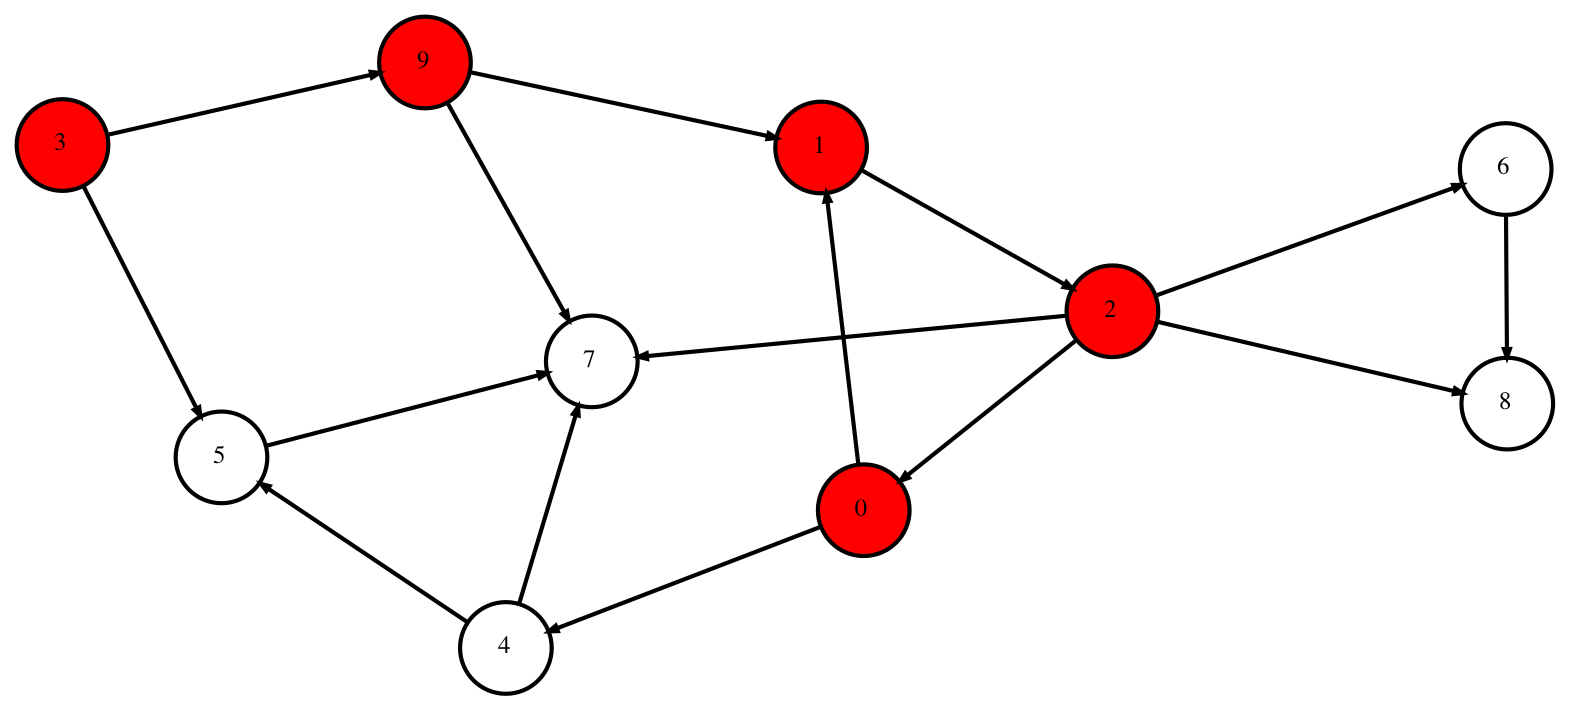
\includegraphics[scale=0.2]{wf.png}
    \caption{Esempio di esecuzione dell'Algoritmo \ref{alg:dfs-wf}. Rosso: \emph{non-well-founded}.}
\end{figure}

Fatte queste premesse introduciamo la funzione ``\rankfunc'', che ricopre un ruolo primario nell'Algoritmo BFA:
\begin{definition}
    Sia $G = (V,E)$ un grafo diretto. Per comodità definiamo le seguenti funzioni:
    \begin{align*}
        &\mathcal{N}_{\scalebox{0.5}{WF}}(n) = \{m \in WF(G) \mid [n] \sccto [m]\}\\
        &\mathcal{N}_{\scalebox{0.5}{NWF}}(n) = \{m \in V - WF(G) \mid [n] \sccto [m]\}
    \end{align*}
    La funzione $\rankfunc: V \to \mathbb{N} \cup \{0, -\infty\}$ è definita come segue:
    \begin{gather*}
        \rankfunc(n) = \begin{cases}
            0 &\text{se $n$ è un pozzo di $G$}\\
            -\infty &\text{se $[n]$ è un pozzo di $G^{\scalebox{.5}{SCC}}$, $n$ non è un pozzo di $G$}\\
            \max(\{1 + \rankfunc(m) \mid m \in \mathcal{N_{\scalebox{0.5}{WF}}}(n)\}\\
            \,\,\,\,\,\,\,\,\,\,\,\,\,\, \cup \,\, \{\rankfunc(m) \mid m \in \mathcal{N_{\scalebox{0.5}{NWF}}}(n)\}) &\text{altrimenti}
        \end{cases}
    \end{gather*}
\end{definition}
\begin{observation}
    Sia $n \in V$, e supponiamo $\rankfunc(n) = k$. Allora $\rankfunc(m) = k$ per ogni vertice nella SCC a cui appartiene $n$.
\end{observation}
\begin{proof2}
    Se $k = 0$, allora $n$ è una foglia, per cui la sua SCC ha cardinalità 1, quindi la tesi vale banalmente. Se $k = -\infty$, nessuno dei nodi in $[n]$ può essere un pozzo di $G$, per cui hanno tutti rango $-\infty$. Quest'ultima argomentazione si può applicare anche al caso in cui $k > 0$, osservando che la definizione della funzione \rankfunc \, non distingue tra nodi appartenenti alla stessa SCC.
\end{proof2}
Se un grafo è \emph{ben fondato}, o se restringiamo il dominio ad un sottografo \emph{ben fondato}, possiamo dare una formulazione alternativa della funzione rank:
\begin{gather*}
        \rankfunc(n) = \begin{cases}
            0 &\text{se $n$ è un pozzo di $G$}\\
            1 + \max\{\rankfunc(m) \mid n E m\} &\text{altrimenti}
        \end{cases}
\end{gather*}
Questa forma sarà utile per semplificare alcune delle dimostrazioni che seguono.

Riportiamo i seguenti risultati da \cite{dovier}, che renderanno più agile l'analisi successiva:
\begin{proposition} \label{prop:rank_bisi_imp_wf}
    Sia $G = (V,E)$. Sia ``\,$\equiv$'' la bisimulazione massima su $G$. Siano $m,n \in WF(G)$. Allora $m \equiv n \implies \rankfunc(m) = \rankfunc(n)$.
\end{proposition}
\begin{proof2}
    Procediamo per induzione su $\rankfunc(m)$. Si ricordi che per il Teorema \ref{theo:bisi_iff_eqsets} $m,n$ rappresentano lo stesso insieme. Se $\rankfunc(m) = 0, m$ rappresenta l'insieme vuoto. Ma allora lo stesso vale per $n$, per cui anche $\rankfunc(n) = 0$.

    Supponiamo che per due nodi bisimili per cui valga $\rankfunc(m) \leq k-1$ valga anche $\rankfunc(m) = \rankfunc(n)$. Sia $\rankfunc(m) = k$, e sia $m' \in V$ il nodo tale che $m E m', \rankfunc(m') = k-1$. Allora deve esistere un nodo $n' \mid n E n', m' \equiv n'$, e quindi $\rankfunc(m') = \rankfunc(n')$. Ma allora $\rankfunc(n) \geq k-1 + 1 = k$, per la formulazione alternativa di rank. Analogamente si dimostra che $\rankfunc(m) \geq k$, per cui si ha la tesi.
\end{proof2}
\begin{proposition}
    \label{prop:omega_rank}
    Sia $G = (V,E)$. Siano $m \in V$. Allora:
    \begin{gather*}
        \rankfunc(m) = -\infty \iff \text{l'APG } \restr{G}{m} \text{rappresenta l'insieme } \Omega
    \end{gather*}
\end{proposition}
\begin{proof2}
    Si ricordi la caratterizzazione dell'insieme $\Omega$ (cioè un insieme che contiene solamente se stesso) fornita in \cite{aczel}: un APG rappresenta $\Omega$ se e solo se ogni nodo ha almeno un arco uscente. Dalle ipotesi fatte si deduce che $[m]$ non contiene solamente $m$ (altrimenti $m$ sarebbe un pozzo di $G$). Possiamo dimostrare che ogni nodo in $[m]$ deve avere almeno un arco uscente: infatti, supponendo che non sia così, tale nodo non avrebbe modo di tornare in $[m]$, per cui non potrebbero stare nella stessa SCC.

    Supponiamo ora che l'APG $\restr{G}{m}$ rappresenti l'insieme $\Omega$. Chiaramente $m$ non può essere un pozzo di $G$, altrimenti non ripetterebbe la caratterizzazione. Supponiamo per assurdo che $[m]$ non sia un pozzo di $G^{\superscc}$, cioè da un nodo di $[m]$ parte un arco verso un nodo $x$. Si presentano quattro possibilità:
    \begin{enumerate}
        \item Da $x$ non esce alcun nodo: impossibile per la caratterizzazione;
        \item Da $x$ esce un unico nodo che ha per destinazione $x$ stesso: $[x]$ contiene solamente $x$, ed è una foglia di $G^{\superscc}$, per cui ha rango $-\infty$;
        \item Da $x$ esce un nodo che ha per destinazione un nodo di $[m]$: impossibile perchè si è supposto $x \not\in [m]$;
        \item Da $x$ esce un nodo che ha per destinazione un nodo $x' \not\in [m]$.
    \end{enumerate}
    Per cui è evidente che le uniche opzioni valide sono b. e d. Possiamo dimostrare che il blocco di $G^{\superscc}$ contenente una sequenza di nodi connessi secondo queste due regole è necessariamente un pozzo: possiamo continuare potenzialmente all'infinito ad aggiungere nuiovi nodi all'infinito, ma l'ultimo nodo dovrà avere un \emph{self loop}, oppure tornare in un nodo precedente della sequenza. In entrambi i casi i nodi coinvolti ottengono rango $-\infty$, per cui a cascata (per il terzo caso nella definizione di \rankfunc) i nodi precedenti della sequenza hanno sempre rango $-\infty$.
\end{proof2}
\begin{proposition}
    Con le stesse ipotesi della Proposizione \ref{prop:rank_bisi_imp_wf}, supponiamo che $m,n \in V - WF(G)$. Allora $m \equiv n \implies \rankfunc(m) = \rankfunc(n)$.
\end{proposition}
\begin{proof2}
    Sempre per il Teorema \ref{theo:bisi_iff_eqsets}, $m,n$ rappresentano lo stesso insieme. Se $\rankfunc(m) = -\infty$, per la proposizione precedente $m$ rappresenta $\Omega$, per cui anche $n$ rappresenta $\Omega$. Ma allora $\rankfunc(n) = -\infty$.

    Se $\rankfunc(m) = h > 0$, per come è stato definita la funzione rank deve esistere un nodo \emph{ben fondato} $m'$ raggiungibile da $m$, non necessariamente in modo diretto, tale che $\rankfunc(m') = h-1$ (il rango aumenta solo in corrispondenza di archi verso nodi \emph{ben fondati}). Poichè $m \equiv n$ deve esistere un nodo \emph{ben fondato} $n'$ raggiungibile da $n$ tale che $m' \equiv n'$. Ma allora ($m',n' \in WF(G)$) $\rankfunc(n') = \rankfunc(m') = h-1$, e quindi $\rankfunc(n) \geq \rankfunc(m) = h$. Analogamente si dimostra che $\rankfunc(m) \geq \rankfunc(n)$, per cui si ha la tesi.
\end{proof2}
\begin{theorem}
    \label{theo:bisi_rank}
    Sia $G = (V,E)$. Sia ``\,$\equiv$'' la bisimulazione massima su $G$. Siano $m,n \in V$. Allora
    \begin{gather*}
        m \equiv n \implies \rankfunc(m) = \rankfunc(n)
    \end{gather*}
\end{theorem}
\begin{proof2}
    \accente chiaro che perchè i nodi possano essere bisimili devono essere entrambi \emph{ben fondati} o entrambi \emph{non ben fondati}. La tesi segue dalle proposizioni appena dimostrate.
\end{proof2}
La funzione \rankfunc \, viene utilizzata dall'Algoritmo BFA per stabilire l'ordine degli \emph{splitter}; giustificheremo in modo dettagliato questa affermazione nel seguito.

Prima di proseguire, proponiamo e commentiamo un algoritmo per la computazione della funzione \rankfunc \, per ogni nodo di un grafo diretto, che verrà usato come subroutine dall'Algoritmo FBA. Avendo a disposizione $G^{\superscc}$, per calcolare il rango dei nodi di $G$ è sufficiente una visita in profondità su $G^{\superscc}$ e su $G$.
\begin{figure}[H]
    \begin{algorithm}[H]
        \label{alg:rank1}
        \KwData{$G = (V,E), G^{\superscc} = (V^{\superscc}, E^{\superscc})$}
        \caption{DFS-Rank}
        \SetAlgoLined
        \SetKwProg{Fn}{function}{:}{end}
        \Fn{\textup{dsf-rank-visit}($G = (V,E), G^{\superscc} = (V^{\superscc},E^{\superscc}), N$)}{
            \uIf{$N = \{n\} \mid$ n è un pozzo di $G$}{
                $N$.rank = 0\;
            }
            \uElseIf{$N$ è un pozzo di $G^{\superscc}$}{
                $N$.rank = $-\infty$\;
            }
            \Else{
                current-max $\coloneqq -\infty$\;
                \ForAll{$M \mid N E^{\superscc} M$}{
                    \lIf*{$M$.rank = NULL}{
                        dfs-rank-visit($G, G^{\superscc}, M$)\;
                    }

                    \eIf{$M = \{m\} \land m.wf$} {
                        current-max = $\max$(current-max, $m$.rank + 1)\;
                    } {
                        current-max = $\max$(current-max, $M$.rank)\;
                    }
                }

                $N$.rank = current-max\;
            }
        }
        \Begin{
            DFS-WF(G)\;

            \While{$\exists N \in V^{\superscc} \mid N.$rank = NULL}{
                dfs-rank-visit($G, G^{\superscc},N$)\;
            }
        }
    \end{algorithm}
\end{figure}

Si osservi che nell'Algoritmo \ref{alg:rank1} non teniamo traccia del colore dei nodi per $G^{\superscc}$, in quanto non c'è il rischio di incontrare cicli. La correttezza è banale, in quanto il rango e $WF(G)$ vengono calcolati semplicemente applicando le definizioni. La complessità (avendo a disposizione $G^{\superscc}$) è chiaramente quella di due visite in profondità, cioè $O(|V| + |E| + |V^{\superscc}| + |E^{\superscc}|) = O(|V| + |E|)$.
\begin{figure}[H]
    \hspace*{-0.8cm}
    \centering
    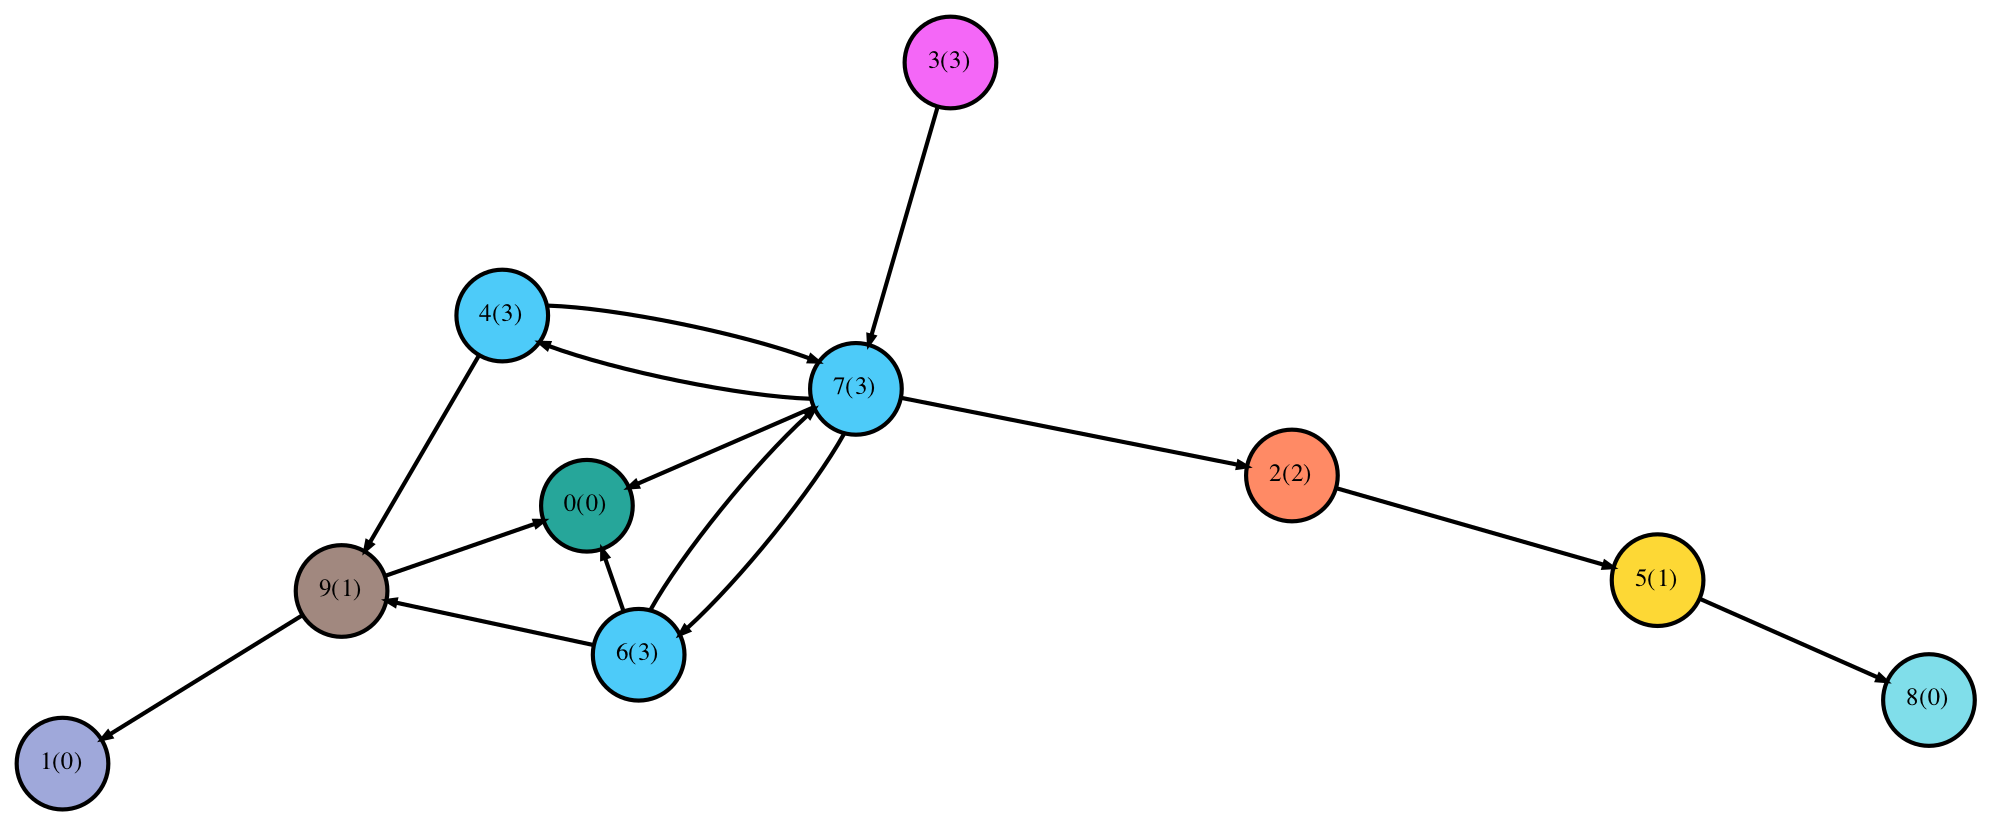
\includegraphics[scale=0.2]{rank.png}
    \caption{Esempio di esecuzione dell'Algoritmo \ref{alg:rank1}. Il rango del nodo è tra parentesi, i nodi appartenenti a diverse SCC sono disegnati in colori diversi.}
\end{figure}

\subsubsection{L'algoritmo}
Per comodità di notazione poniamo $\mathbb{N}^* \coloneqq \mathbb{N} \cup \{-\infty, 0\}$. Presentiamo lo pseudocodice per l'Algoritmo FBA:\\
\begin{algorithm}[H]
    \label{alg:fba}
    \KwData{$G = (V,E)$}
    \caption{Algoritmo FBA}
    \SetKwProg{Fn}{function}{:}{end}
    \Fn{\textup{collapse}($G = (V,E), B \subseteq V$)}{
        Sia $u \in V$ scelto casualmente\;
        \ForAll{$v \in B$}{
            \ForAll{$e \in E \mid$ ``$e$ è incidente a $v$''}{
                \tcp*[h]{$e'$ è l'arco $e$ se si sostuisce $u$ al posto di $v$}\\
                $E = (E - \{e\}) \cup \{e'\}$\;
            }
            $V = V - \{v\}$\;
        }
        \Return{$u$}\;
    }
    \Fn{\textup{Split2}($G = (V,E), P, u, \widehat{B}$)} {
        \ForAll{$B \in P \mid B \in \widehat{B}$}{
            $P = (P - \{B\}) \cup \{\{v \in B \mid v E u\}, \{v \in B \mid \neg (v E u)\}\}$\;
        }
    }
    \Begin{
        DFS-RANK($G$)\;
        $\rho \coloneqq \max\{\rankfunc(n) \mid n \in V\}$\;
        $B_k \coloneqq \{n \in V \mid \rankfunc(n) = k\}, \,\, k \in \mathbb{N}^*$\;
        $P \coloneqq \{B_i \mid i \in \mathbb{N}^*\}$\; \label{alg:partizione_rudimentale}

        \tcp*[h]{$u$ è il nodo di $B_{-\infty}$ preservato da collapse}\\
        $u  \coloneqq$ collapse($G,B_{-\infty}$)\; \label{alg:impunemente_omega}
        Split2($G, P, u, \bigcup_{i=0}^\rho B_i$)\; \label{alg:split_post_omega}

        \ForAll{$i = 0, \dots, \rho$}{
            \tcp*[h]{i blocchi di $P$ aventi rango $i$}\\
            $D_i \coloneqq \{B \in P \mid B \subseteq B_i\}$\;
            Sia $\restr{G}{i}$ come nella Definizione \ref{def:grafo_restr}\,\;
            \tcp*[h]{$D_i$ è una partizione di $G_i$}\\
            $D_i =$ Paige-Tarjan($G_i, D_i$)\;

            \ForAll{$B \in D_i$}{
                $u \coloneqq$ collapse($G,B$)\;
                Split2($G, P, u, \bigcup_{j=i+1}^\rho B_i$)\;
            }
        }
    }
\end{algorithm}

La funzione ``collapse'' rimuove dal grafo tutti i nodi all'interno di un blocco, ad eccezione di un nodo scelto in modo casuale. Dopodichè sostituisce il nodo mantenuto nel ruolo dei nodi rimossi in ogni arco incidente ad un nodo rimosso. Questa funzione viene usata per contrarre i nodi in un blocco per cui si è già stabilito che siano tutti bisimili. La funzione ``Split2'' è analoga alla funzione ``\splitfunc'', ma consente di specificare i blocchi che possono essere divisi (cioè solo quelli in $\widehat{B}$), e prende in considerazione un unico vertice (cioè $u$) come destinazione degli archi partenti dai blocchi in $\widehat{B}$.

L'algoritmo inizia con il calcolo del rango dei nodi del grafo. Alla Riga \ref{alg:partizione_rudimentale} viene creata una partizione iniziale, da rifinire, i cui blocchi sono composti dai nodi aventi lo stesso rango. Per il Teorema \ref{theo:bisi_rank} sarà sicuramente necessario rifinire questa partizione per determinare la bisimulazione massima: non è possibile infatti che vi siano due nodi bisimili che vengono sistemati in due blocchi differenti a questo punto.

Per la Proposizione \ref{prop:omega_rank} possiamo impunemente considerare bisimili tutti i nodi di rango $-\infty$. Per questo motivo alla Riga \ref{alg:impunemente_omega} viene ``collassato'' il blocco $B_\infty$. Si noti che un'assunzione del genere non è valida per altri valori del rango, in quanto nodi non bisimili possono avere lo stesso rango. A questo punto è necessario aggiornare la partizione e dividere ogni blocco che non rispetta la condizione di stabilità (Riga \ref{alg:split_post_omega}).

In seguito, per ogni rango a partire 0, si considerano i blocchi di rango $i$ e si isola il sottografo contenente solamente nodi composti dai nodi che vi sono contenuti. Si applica l'algoritmo PTA a questo sottografo, in modo da calcolarne la RSCP. I blocchi di questa nuova partizione vengono ``collassati'', ed analogamente a quanto fatto in precedenza si impone ai blocchi di rango superiore la condizione di stabilità.

\subsubsection{Correttezza e complessità}
Siano $m,n \in V \mid m \equiv n$. Per il Teorema \ref{theo:bisi_rank} $m,n$ devono necessariamente stare all'interno dello stesso blocco nella partizione iniziale creata alla Riga \ref{alg:partizione_rudimentale}. Dimostriamo ora che durante l'esecuzione dell'algoritmo non vengono mai divisi.
